% Texto adaptado de docs/tcc2/relatorio_tcc2.md para a prévia do TCC2.
\chapter{Desenvolvimento e resultados}\label{cap:tcc2-5}

Este capítulo apresenta o produto desenvolvido e os resultados disponíveis. A primeira parte descreve a experiência do ponto de vista do jogador, funcionando como um guia conciso do jogo entregue. A segunda constitui o relatório técnico, no qual são discutidas a arquitetura, a sincronização e a implementação das principais funcionalidades. A parte final reúne a verificação funcional, os resultados das métricas, a comparação com a proposta e as limitações identificadas.

\section{Visão geral do jogo final}\label{sec:5.1}

Esta seção apresenta o jogo conforme percebido pelo participante, desde a entrada em uma partida até a exibição do resultado. Os detalhes internos que sustentam esse funcionamento são discutidos posteriormente, no relatório técnico.

\subsection{Conceito e ciclo principal de jogabilidade}\label{sec:5.1.1}

O jogo desenvolvido organiza confrontos entre duas equipes em uma arena tridimensional. O participante informa seu nome, seleciona um preset e aguarda a formação da partida. Após o carregamento do mapa e a escolha de arma, passa a controlar seu personagem, podendo buscar recursos, enfrentar o adversário e disputar o objetivo do modo. A partida termina conforme suas regras, e uma tela apresenta os resultados por equipe e por jogador. \fonteprojeto{PRESETS} \fonteprojeto{SERVER} \fonteprojeto{SERVER-LOBBY} \fonteprojeto{MENU} \fonteprojeto{RESULTADO}

O ciclo de interação combina deslocamento, gerenciamento de munição e confronto. Ao perder todos os pontos de vida, o personagem é removido e, caso a partida continue, o jogador recebe uma nova oportunidade de escolher sua arma e retornar ao mapa. Dessa forma, a participação se organiza em torno da disputa em andamento. O inventário é preparado novamente no nascimento, sem representar uma progressão persistente entre partidas. \fonteprojeto{SERVER-LOBBY} \fonteprojeto{INVENTARIO}

\subsection{Controles e movimentação}\label{sec:5.1.2}

A movimentação foi implementada no Client por meio de um corpo tridimensional controlado por script. A direção é calculada a partir da entrada e da orientação do personagem. A câmera permite olhar horizontal e verticalmente, com limitação da rotação vertical. O jogador pode correr e realizar até dois saltos antes de retornar ao chão. A implementação também considera a entrada por controle, incluindo deslocamento e mira pelos analógicos. \fonteprojeto{JOGADOR-LOCAL} \fonteprojeto{PROJETO-CLIENT}

O salto duplo é controlado por uma contagem de saltos utilizados. Quando o personagem aterrissa, essa contagem é reiniciada; ao tocar uma plataforma de impulso, a velocidade vertical é alterada e os saltos também são restabelecidos. Os jump pads são configurados pelo Server e apresentados no Client, onde a detecção de contato aplica o impulso ao personagem local. O Server recebe depois a posição resultante pelo fluxo normal de movimento; não há uma validação separada de cada impulso na implementação consultada. \fonteprojeto{JOGADOR-LOCAL} \fonteprojeto{JUMP-PAD} \fonteprojeto{SERVER-LOBBY}

\begingroup
\small
\setlength{\tabcolsep}{4pt}
\renewcommand{\arraystretch}{1.18}
\begin{longtable}{>{\raggedright\arraybackslash}p{\dimexpr0.23\textwidth-2\tabcolsep\relax}>{\raggedright\arraybackslash}p{\dimexpr0.35\textwidth-2\tabcolsep\relax}>{\raggedright\arraybackslash}p{\dimexpr0.42\textwidth-2\tabcolsep\relax}}
\caption{Principais controles presentes na configuração do Client}\label{tab:tcc2-2}\\
\toprule
Ação & Teclado e mouse & Controle, em nomenclatura equivalente à disposição Xbox \\
\midrule
\endfirsthead
\multicolumn{3}{l}{\small Principais controles presentes na configuração do Client (continuação)}\\
\toprule
Ação & Teclado e mouse & Controle, em nomenclatura equivalente à disposição Xbox \\
\midrule
\endhead
\midrule
\multicolumn{3}{r}{\small Continua na próxima página.}\\
\endfoot
\bottomrule
\endlastfoot
Movimentar & W, A, S e D & Analógico esquerdo \\
Mirar & Movimento do mouse & Analógico direito \\
Correr & Shift & Pressionar o analógico esquerdo \\
Saltar & Espaço & A \\
Disparar & Botão esquerdo do mouse & Gatilho direito ou botão superior direito \\
Lançar granada & Q & Botão superior esquerdo ou B \\
Selecionar arma & 1, 2 e 3 & Direcional esquerdo/direito para alternar \\
Abrir ou fechar pausa & Esc & Start/Menu \\
\end{longtable}
\endgroup

Fonte: Input Map e tratamento de entrada do Client. O mapeamento documenta a configuração existente; a verificação em dispositivos físicos integra o teste da release. \fonteprojeto{PROJETO-CLIENT} \fonteprojeto{JOGADOR-LOCAL} \fonteprojeto{GUIA-RELEASE}

\subsection{Fluxo de telas}\label{sec:5.1.3}

O gerenciador de cenas abre o menu principal quando o Client inicia. A formação da partida conduz ao carregamento do mapa e à seleção de arma; durante o jogo, a pausa disponibiliza uma tela local e libera o cursor. Esse estado interrompe o controle daquele jogador, mas não suspende o processo servidor. Ao final da partida, os dados recebidos são entregues à tela de resultado, que permite voltar ao menu. A Figura~\ref{fig:tcc2-1} resume esse encadeamento. \fonteprojeto{CENAS-CLIENT} \fonteprojeto{JOGADOR-LOCAL} \fonteprojeto{CLIENT-LOBBY} \fonteprojeto{RESULTADO}

\begin{figure}[htbp]
\centering
\caption{Fluxo principal de telas e participação}
\label{fig:tcc2-1}
% Fluxo de telas do jogo.
\resizebox{0.96\linewidth}{!}{%
\begin{tikzpicture}[
  bloco/.style={draw,rounded corners,align=center,text width=2.8cm,minimum height=.75cm,font=\small},
  seta/.style={-{Latex[length=2mm]},thick}
]
\node[bloco] (menu) at (0,0) {Menu principal};
\node[bloco] (espera) at (0,-1.2) {Espera por partida};
\node[bloco] (mapa) at (0,-2.4) {Carregamento do mapa};
\node[bloco] (arma) at (0,-3.6) {Seleção de arma};
\node[bloco] (partida) at (0,-4.8) {Partida e HUD};
\node[bloco] (pausa) at (-4,-4.8) {Pausa local};
\node[bloco] (morte) at (4,-4.8) {Morte e espera};
\node[bloco] (resultado) at (0,-6.2) {Resultado};
\draw[seta] (menu) -- (espera);
\draw[seta] (espera) -- (mapa);
\draw[seta] (mapa) -- (arma);
\draw[seta] (arma) -- (partida);
\draw[seta] (partida) to[bend right=15] (pausa);
\draw[seta] (pausa) to[bend right=15] (partida);
\draw[seta] (partida) -- (morte);
\draw[seta] (morte) |- (arma);
\draw[seta] (partida) -- (resultado);
\draw[seta] (resultado.south) -- ++(0,-.6) -- (-6,-6.8) -- (-6,0) -- (menu.west);
\end{tikzpicture}%
}

\fonte{elaboração a partir dos gerenciadores de cena e lobby. O retorno após a morte depende de a partida continuar ativa. \fonteprojeto{CENAS-CLIENT} \fonteprojeto{CLIENT-LOBBY} \fonteprojeto{SERVER-LOBBY}}
\end{figure}

\subsection{Modos de jogo e objetivos}\label{sec:5.1.4}

O jogador pode participar de Team Deathmatch ou King of the Hill. No primeiro modo, as equipes disputam pontos por meio das eliminações, e quedas que provoquem a morte também favorecem a equipe adversária. No segundo, o objetivo é ocupar a zona demarcada no mapa: uma equipe pontua enquanto controla sozinha a região, e a progressão é interrompida quando adversários entram na área. \fonteprojeto{TDM} \fonteprojeto{KOTH} \fonteprojeto{COLINA} \fonteprojeto{ZONA-MORTE}

Nos presets disponíveis, as partidas utilizam meta de 20 pontos e duração máxima de 300 segundos. Ao atingir a meta ou terminar o tempo, o jogo apresenta a equipe vencedora e os dados individuais dos participantes. \fonteprojeto{PRESETS} \fonteprojeto{RESULTADO}

\subsection{Armas, granadas e recursos da arena}\label{sec:5.1.5}

O arsenal é formado por pistola, SMG e shotgun. A pistola realiza disparos individuais, a SMG permite manter o gatilho pressionado e a shotgun dispara vários traços simultaneamente. O jogador escolhe uma arma antes de entrar ou retornar à arena e precisa administrar sua munição durante a partida. Também pode lançar granadas, que explodem após um intervalo e causam dano de acordo com a distância. \fonteprojeto{ARMAS} \fonteprojeto{PISTOLA} \fonteprojeto{SMG} \fonteprojeto{SHOTGUN} \fonteprojeto{GRANADA-SERVER}

O mapa distribui pickups de vida, munição e granadas, além de dois power-ups temporários. Um deles aumenta o dano dos disparos e o outro reduz o intervalo entre tiros. Depois de coletados, os recursos permanecem indisponíveis por um período antes de reaparecerem. \fonteprojeto{PICKUPS} \fonteprojeto{BUFF-DANO} \fonteprojeto{BUFF-CADENCIA}

\subsection{Interface e feedback ao jogador}\label{sec:5.1.6}

A HUD informa vida, equipe, arma equipada, munição, granadas e efeitos temporários. Durante a partida, também apresenta o tempo, o placar e, em KOTH, o estado da zona de controle. Cores, anéis e ícones auxiliam na identificação das equipes. \fonteprojeto{HUD-CENA} \fonteprojeto{JOGADOR-LOCAL} \fonteprojeto{CLIENT-LOBBY}

Sons, recuo, efeitos de disparo e impacto e alterações visuais dos personagens complementam essas informações. Esses sinais permitem perceber a ocorrência de ações como disparos, coletas, explosões e recebimento de dano sem depender exclusivamente de mensagens textuais. \fonteprojeto{AUDIO} \fonteprojeto{DISPARO-LOCAL} \fonteprojeto{PERSONAGEM} \fonteprojeto{ROSTO}

\section{Relatório técnico}\label{sec:5.2}

Esta seção concentra a descrição do desenvolvimento. A organização acompanha as responsabilidades e relações entre os sistemas, utilizando as funcionalidades como exemplos da solução técnica em vez de enumerar arquivos e classes.

\subsection{Separação entre Client, Server e shared}\label{sec:5.2.1}

O sistema foi dividido para que apresentação e regras de partida pudessem ser executadas em processos diferentes. O Client recebe a entrada, movimenta o personagem local e apresenta modelos, sons e interface. O Server organiza os participantes e mantém os estados utilizados no combate, na coleta de itens e na pontuação. O diretório \texttt{shared} contém definições comuns, evitando que identificadores e regras como os limites de munição sejam mantidos de forma independente nos dois projetos. \fonteprojeto{DOC-ARQUITETURA} \fonteprojeto{DOC-SHARED} \fonteprojeto{INVENTARIO}

\begin{figure}[htbp]
\centering
\caption{Responsabilidades dos componentes. \texttt{shared} é um diretório de código e recursos, e não um serviço da rede}
\label{fig:tcc2-2}
% shared representa arquivos usados pelos dois projetos, não um serviço.
\resizebox{0.96\linewidth}{!}{%
\begin{tikzpicture}[
  bloco/.style={draw,rounded corners,align=center,text width=4.5cm,minimum height=1.3cm,font=\small},
  seta/.style={-{Latex[length=2mm]},thick}
]
\node[bloco] (client) at (-4,0) {Client\\Entrada, movimento local\\e apresentação};
\node[bloco] (server) at (4,0) {Server\\Lobbies, combate,\\recursos e modos};
\node[bloco] (shared) at (0,3.1) {shared\\Contratos, presets e definições};
\draw[seta] (client.north east) -- node[above,align=center,font=\footnotesize] {Estado local\\e solicitações} (server.north west);
\draw[seta] (server.south west) -- node[below,font=\footnotesize] {Snapshots e eventos} (client.south east);
\draw[seta,dashed] (shared) -- node[left,font=\footnotesize] {Usado pelo código} (client);
\draw[seta,dashed] (shared) -- node[right,font=\footnotesize] {Usado pelo código} (server);
\end{tikzpicture}%
}

\fonte{organização dos projetos e fluxo dos lobbies. \fonteprojeto{DOC-SHARED} \fonteprojeto{CLIENT-LOBBY} \fonteprojeto{SERVER-LOBBY}}
\end{figure}

\subsection{Comunicação e autoridade do servidor}\label{sec:5.2.2}

O disparo exemplifica essa divisão. O Client apresenta o efeito local e envia a solicitação. O Server verifica se o jogador possui uma instância ativa, identifica a arma registrada e tenta consumir a munição correspondente. Se houver saldo, calcula os acertos e aplica o dano. As alterações de vida e os efeitos de impacto são então comunicados aos participantes. A apresentação imediata do disparo não concede ao Client a responsabilidade de decidir quem foi atingido. \fonteprojeto{DISPARO-LOCAL} \fonteprojeto{SERVER-LOBBY} \fonteprojeto{CLIENT-LOBBY}

A autoridade implementada possui limites. O Server aceita a transformação enviada pelo jogador após verificar a estrutura da mensagem, e o caminho de recepção do disparo não contém uma verificação explícita de intervalo mínimo entre solicitações. O cooldown e seu multiplicador de cadência são aplicados no Client. Assim, dano e munição são decididos no Server, mas a versão atual não equivale a uma validação completa de movimento e frequência de tiro contra um Client modificado. \fonteprojeto{SERVER-LOBBY} \fonteprojeto{DISPARO-LOCAL} \fonteprojeto{PERSONAGEM}

\subsection{Sessões, lobbies e presets de partida}\label{sec:5.2.3}

Uma conexão ao servidor e a participação em uma partida são estados diferentes. O Server recebe conexões e procura um lobby disponível para o preset solicitado. Quando necessário e permitido pelo limite configurado, cria outro lobby; quando o grupo está completo, inicia a preparação dos Clients. Os presets agrupam modo, mapa, tempo, pontuação e quantidade de participantes, tornando a configuração conhecida pelos dois lados. \fonteprojeto{SERVER} \fonteprojeto{PRESETS}

Na configuração consultada, o peer aceita até 64 conexões, o gerenciador possui quatro posições de lobby e cada preset utiliza dois jogadores. Portanto, o limite de conexões não significa 64 jogadores na mesma partida. Cada lobby mantém seus próprios participantes e estado, e suas cenas são posicionadas com uma separação espacial no processo servidor. A comprovação de execução simultânea dos quatro lobbies exige um cenário de avaliação próprio. \fonteprojeto{SERVER} \fonteprojeto{PRESETS} \fonteprojeto{SERVER-LOBBY}

\subsection{Sincronização de rede}\label{sec:5.2.4}

\textbf{Envio contínuo de movimento.} A cada ciclo de física, o Client envia posição, rotação horizontal, inclinação da mira e animação. O Server copia esses dados para a representação do jogador e os utiliza na composição do estado da partida. Esse envio emprega o modo não confiável ordenado, adequado ao tratamento de informações que serão substituídas por novas atualizações. O fluxo transmite o resultado local do movimento, em vez de uma sequência de comandos para o Server simular novamente. \fonteprojeto{CLIENT-LOBBY} \fonteprojeto{SERVER-LOBBY}

\subsubsection{Interpolação dos estados remotos}\label{sec:5.2.4.1}

O Server distribui snapshots do estado do mundo a cada três ciclos de física, enquanto o Client produz novos quadros continuamente. Como o tempo de trânsito pela rede pode variar, os snapshots podem chegar em intervalos irregulares. Se cada quadro utilizasse apenas o estado mais recente, uma renderização poderia ocorrer antes da chegada da atualização seguinte, mantendo temporariamente a última posição conhecida ou exigindo uma estimativa do movimento. \fonteprojeto{SERVER-LOBBY} \fonteprojeto{CLIENT-LOBBY}

Para reduzir essas descontinuidades, o Client mantém um buffer e calcula um instante de apresentação 100 milissegundos no passado. O desvio estimado entre os relógios do Client e do Server também participa desse cálculo. A cada quadro, o sistema procura dois estados conhecidos ao redor do instante de apresentação e interpola entre eles as posições e rotações dos jogadores remotos. \fonteprojeto{CONEXAO-CLIENT} \fonteprojeto{CLIENT-LOBBY} \fonteprojeto{JOGADOR-REMOTO}

A Figura~\ref{fig:tcc2-3} compara os dois casos com o mesmo conjunto de snapshots disponíveis, posicionados na linha do tempo pelo timestamp do Server, e não pelo instante de chegada ao Client. Sem atraso de apresentação, o instante desejado de 10,000 segundos está além do último estado conhecido, sem um estado posterior para formar o par de interpolação. Com o buffer de 100 milissegundos, o instante de apresentação $R$ passa a ser 9,900 segundos, entre os estados S1 e S2, permitindo calcular uma posição intermediária. Os valores temporais do diagrama são ilustrativos.

\begin{figure}[htbp]
\centering
\caption[Interpolação de snapshots com buffer de apresentação]{Interpolação de snapshots: comparação entre a apresentação sem atraso e com buffer de 100 milissegundos}
\label{fig:tcc2-3}
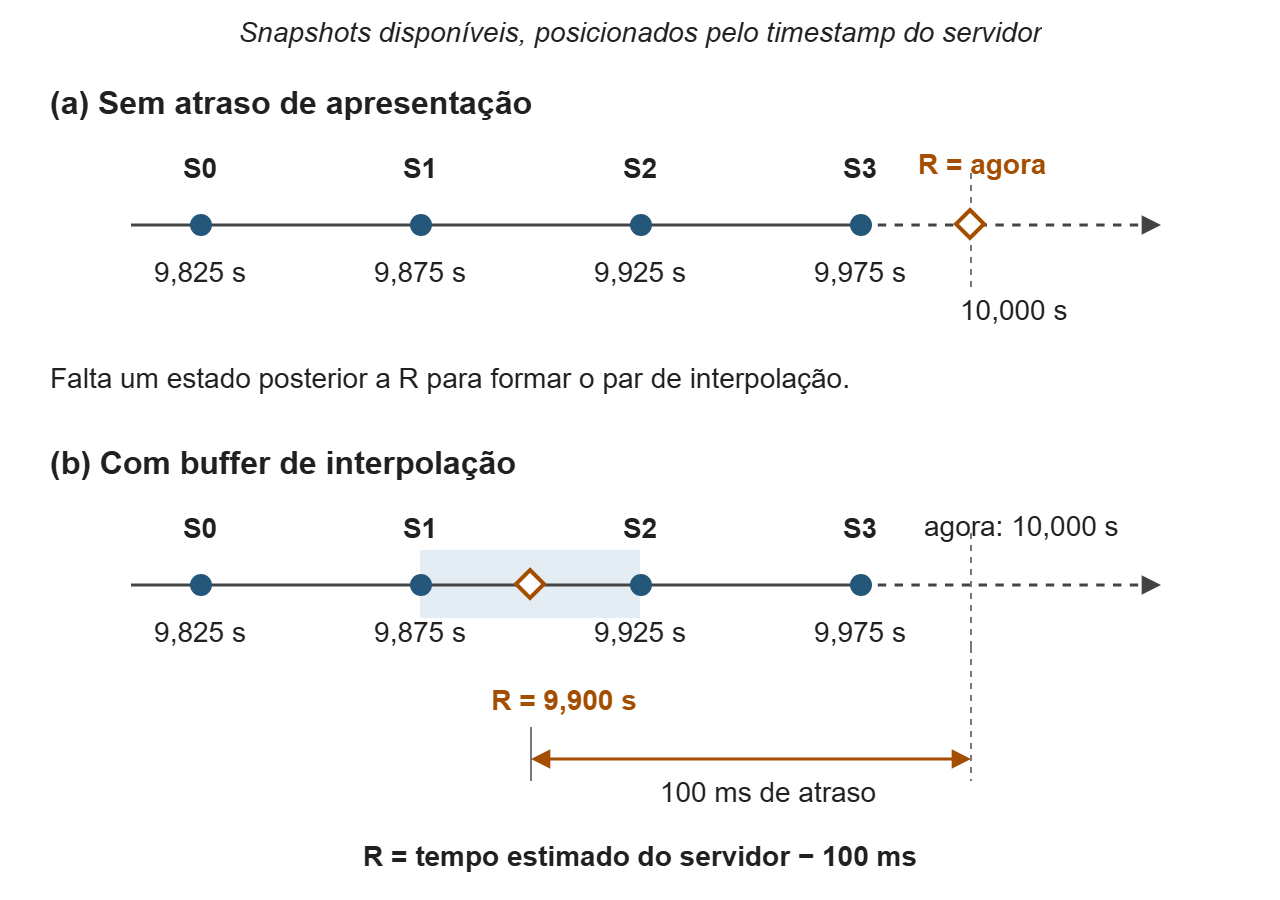
\includegraphics[width=\linewidth,height=0.70\textheight,keepaspectratio]{figuras/tcc2/interpolacao-snapshots.png}
\fonte{elaboração própria a partir da implementação. \fonteprojeto{CLIENT-LOBBY}}
\end{figure}

O atraso de 100 milissegundos é intencional e pertence à apresentação visual; ele não representa uma medição da latência da conexão. Essa estratégia troca uma pequena quantidade fixa de atraso por maior continuidade visual. Na implementação atual, o fator de interpolação não é limitado explicitamente ao intervalo entre zero e um. Caso não exista um estado posterior adequado, o cálculo não garante que o resultado permaneça estritamente entre os dois snapshots utilizados. \fonteprojeto{CLIENT-LOBBY}

\subsubsection{Compensação de latência dos disparos}\label{sec:5.2.4.2}

A interpolação melhora a apresentação dos jogadores remotos, mas não resolve o intervalo entre um disparo no Client e seu processamento pelo Server. Durante esse período, um alvo pode se deslocar. Se o raycast fosse executado somente contra a posição corrente no momento da recepção, um disparo alinhado com aquilo que o atirador viu poderia ser considerado uma falha.

Ao disparar, o Client envia uma referência temporal ajustada pelo desvio estimado entre os relógios. O Server mantém um histórico recente dos estados e, ao receber a solicitação, subtrai os 100 milissegundos do buffer de apresentação para determinar o instante que se aproxima daquele exibido ao atirador. Em seguida, reposiciona as representações auxiliares dos jogadores com os dados históricos, aguarda um ciclo de física e executa o raycast nessa configuração. \fonteprojeto{CONEXAO-CLIENT} \fonteprojeto{CLIENT-LOBBY} \fonteprojeto{SERVER-LOBBY}

A Figura~\ref{fig:tcc2-4} ilustra o processo com todos os instantes expressos na referência temporal do Server. O Client dispara em 10,000 segundos enquanto apresenta aproximadamente o estado A, associado a 9,900 segundos. No exemplo, a solicitação leva 60 milissegundos para chegar ao Server, que já está no estado C em 10,060 segundos. A consulta histórica utiliza o timestamp do disparo menos o buffer visual, isto é, $10{,}000 - 0{,}100 = 9{,}900$ segundos, e não o instante de recepção menos esse buffer. Os 60 milissegundos representam apenas o trânsito de ida em um exemplo ilustrativo, não uma medição nem o tempo de ida e volta da conexão. O estado histórico selecionado aproxima a situação apresentada ao atirador; a implementação não interpola os estados desse histórico.

\begin{figure}[htbp]
\centering
\caption[Compensação de latência na validação de disparos]{Compensação de latência: relação entre o disparo, a recepção e a consulta histórica para validação por raycast}
\label{fig:tcc2-4}
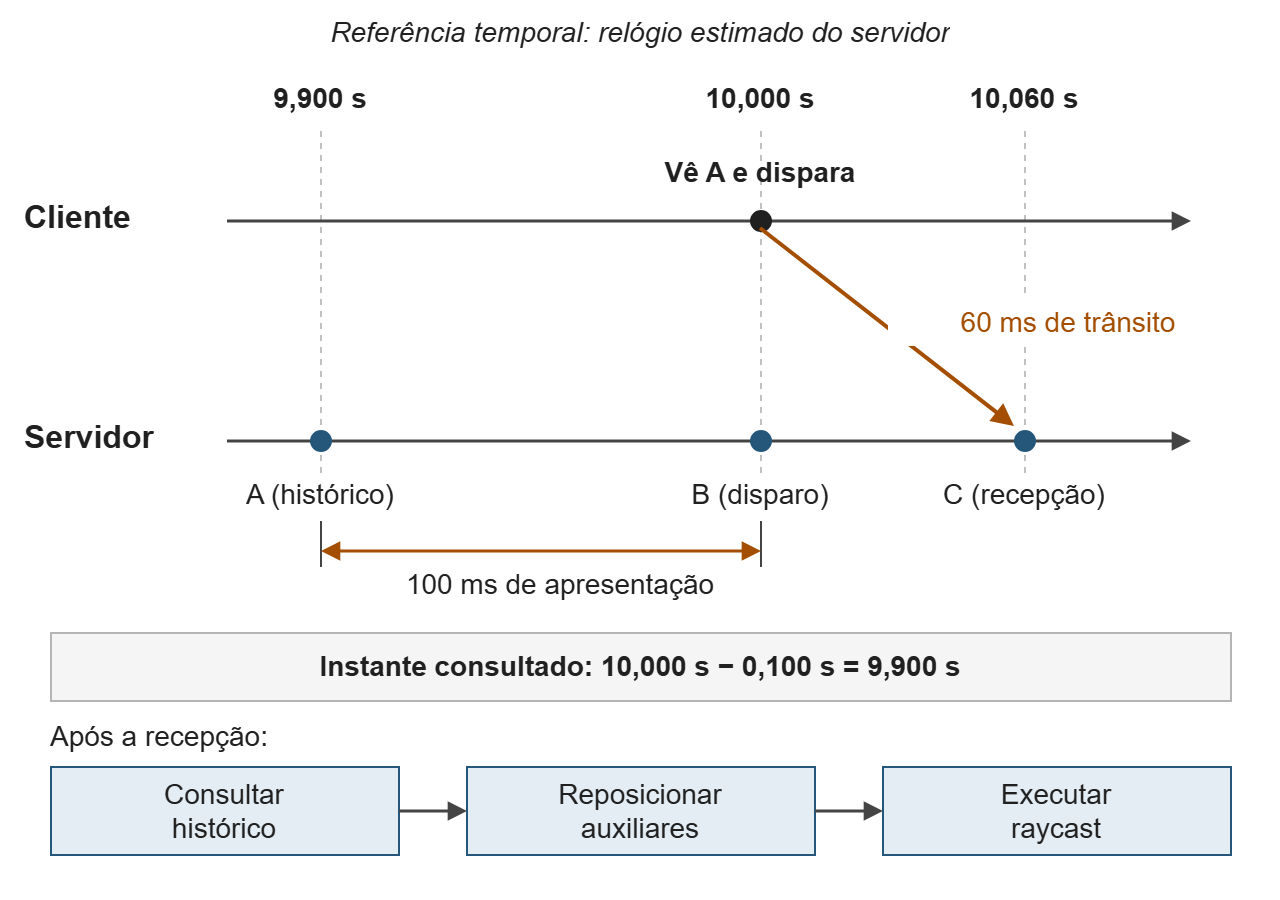
\includegraphics[width=\linewidth,height=0.70\textheight,keepaspectratio]{figuras/tcc2/compensacao-latencia-disparos.png}
\fonte{elaboração própria a partir da implementação. \fonteprojeto{SERVER-LOBBY}}
\end{figure}

Esse procedimento pode ser entendido como uma consulta ao passado para validar o disparo, mas não realiza um rollback completo da partida. O estado corrente do mundo não é integralmente reconstruído nem simulado novamente. Somente as representações auxiliares usadas nos testes de colisão são reposicionadas a partir do histórico recente. O mecanismo busca aproximar a decisão autoritativa da situação vista pelo jogador, sem garantir sincronização exata entre os relógios. \fonteprojeto{SERVER-LOBBY} \fonteprojeto{CONEXAO-CLIENT}

\textbf{Sincronização inicial do mapa.} O Client recebe o identificador do mapa e carrega sua cena local. Após confirmar o carregamento, recebe mensagens confiáveis para criar pickups, objetivos e plataformas especiais. São enviados identificadores e parâmetros de criação, sem retransmitir continuamente toda a geometria visual. Assim, a posição inicial da zona de KOTH e dos jump pads faz parte da preparação da partida. \fonteprojeto{SERVER-LOBBY} \fonteprojeto{CLIENT-LOBBY} \fonteprojeto{PAYLOADS}

\textbf{Atualizações do objetivo.} A criação inicial da zona de controle não elimina a necessidade de comunicar suas mudanças. O KOTH verifica a ocupação durante a execução e transmite o estado da colina a cada 0,25 segundo. A mensagem contém a condição da zona, o time controlador e os jogadores presentes. O placar possui outro fluxo de atualização, permitindo distinguir a existência do objetivo, seu estado atual e a pontuação acumulada. \fonteprojeto{KOTH} \fonteprojeto{COLINA} \fonteprojeto{CLIENT-LOBBY}

\textbf{Eventos confiáveis.} Nascimento, troca de arma, início e término de power-ups e encerramento da partida são comunicados por eventos confiáveis. Nesses casos, a mudança é transmitida quando ocorre, com os dados necessários à atualização da cópia local. O objetivo é preservar a entrega e a ordem enquanto a conexão permanece válida; isso não constitui, por si só, um mecanismo de persistência ou recuperação após desconexão. \fonteprojeto{SERVER-LOBBY} \fonteprojeto{CLIENT-LOBBY} \cite{GODOT-PEER}

\textbf{Predição local e correção de munição.} Ao disparar, o Client reduz sua munição, inicia o cooldown e apresenta recuo, som e efeito de tiro antes da resposta do Server. O valor confirmado pelo servidor substitui a cópia local quando é recebido. Essa antecipação produz uma resposta imediata, mas a implementação não mantém um histórico de comandos confirmados para repetir toda a simulação do personagem. Trata-se de uma correção de estado discreto associada ao disparo. \fonteprojeto{DISPARO-LOCAL} \fonteprojeto{JOGADOR-LOCAL} \fonteprojeto{SERVER-LOBBY}

\textbf{Granadas por snapshots.} As granadas são simuladas fisicamente no Server e identificadas por um código de rede. O Client cria sua representação quando o identificador aparece nos snapshots e interpola as transformações recebidas. A explosão visual ocorre quando a granada desaparece entre dois estados consecutivos. Embora o Server também envie uma notificação confiável de explosão, o handler atual dessa notificação está vazio no Client; a apresentação efetiva depende da transição dos snapshots. \fonteprojeto{GRANADA-SERVER} \fonteprojeto{SERVER-LOBBY} \fonteprojeto{CLIENT-LOBBY}

\textbf{Reenvio do estado atual.} Além das atualizações individuais, o Server pode enviar o inventário completo de munição e os power-ups ativos. No caso de um buff já em andamento, a mensagem de reenvio utiliza duração zero. O Client aplica os multiplicadores e a apresentação do efeito, mas o personagem local somente inicia um temporizador de HUD quando recebe uma duração positiva. Esse fluxo repõe informações atuais sem repetir as coletas anteriores e sem reconstruir o tempo restante do indicador. \fonteprojeto{SERVER-LOBBY} \fonteprojeto{PERSONAGEM} \fonteprojeto{JOGADOR-LOCAL}

\textbf{Eventos visuais e dados substituíveis.} Efeitos remotos de tiro, impacto e coleta utilizam mensagens não confiáveis. Vida, quantidade de granadas e tempo de partida possuem atualizações não confiáveis ordenadas. A perda de uma mensagem de apresentação não modifica o estado calculado no Server, mas pode deixar um indicador desatualizado até uma comunicação posterior. No caso da vida, por exemplo, não se deve presumir uma correção periódica independente se nenhuma nova atualização ocorrer. \fonteprojeto{SERVER-LOBBY} \fonteprojeto{CLIENT-LOBBY}

\textbf{Variações visuais locais.} O time do jogador é enviado na mensagem de criação, mas a variante de cor da skin não faz parte desse contrato. Cada Client escolhe uma cor da paleta correspondente ao criar sua representação remota. Por isso, o mesmo personagem pode ter tonalidades diferentes em computadores distintos. O anel utiliza um material fixo para cada equipe, mantendo essa identificação vinculada ao time recebido. \fonteprojeto{PAYLOADS} \fonteprojeto{JOGADOR-REMOTO}

\textbf{Comparação com simulação determinística e catch-up.} O material Network Weapon with netfox apresenta uma alternativa em que projéteis avançam por passos determinísticos, recuperam passos perdidos por catch-up e reconciliam a posição inicial com a autoridade usando um limiar de distância. Essas estratégias servem como referência conceitual, mas não descrevem os tiros deste projeto: suas armas usam raycasts históricos, e as granadas recebem transformações periódicas. Não se deve confundir a compensação histórica de um acerto com a execução acelerada de passos de um projétil. \cite{NETFOX} \fonteprojeto{SERVER-LOBBY}

\subsection{Jogador, times e ciclo de vida}\label{sec:5.2.5}

Cada participante possui uma representação local em seu Client e representações remotas nos demais. O Server mantém os dados utilizados na partida, incluindo time, arma, vida e estatísticas. A criação transmite essas informações para que cada Client instancie o tipo de personagem adequado. O jogador remoto combina animação corporal e orientação da mira para apresentar o estado recebido pela rede. \fonteprojeto{SERVER-LOBBY} \fonteprojeto{CLIENT-LOBBY} \fonteprojeto{JOGADOR-REMOTO}

A identificação das equipes utiliza materiais do personagem, um anel e um ícone na HUD do jogador local. O ícone permite consultar o próprio time sem depender de enxergar o corpo do personagem em primeira pessoa. As variações de skin permanecem locais, conforme descrito na seção anterior, enquanto a equipe utilizada pelas regras é definida no Server. \fonteprojeto{JOGADOR-REMOTO} \fonteprojeto{JOGADOR-LOCAL}

O jogador possui vida máxima de 100 pontos. Quando o valor chega a zero, o Server remove suas representações, retira sua presença dos objetivos e limpa os power-ups. Se a partida continuar, aguarda cinco segundos antes de solicitar uma nova escolha de arma. O retorno ocorre com a preparação do estado de nascimento e da munição correspondente à escolha, sem um contador de vidas limitado nos presets atuais. \fonteprojeto{JOGADOR-SERVER} \fonteprojeto{SERVER-LOBBY} \fonteprojeto{INVENTARIO} \fonteprojeto{PRESETS}

\subsection{Modos de jogo e fluxo da partida}\label{sec:5.2.6}

\textbf{Team Deathmatch.}

No Team Deathmatch, o objetivo é obter a maior pontuação no confronto entre equipes. Na implementação, a pontuação de cada time corresponde à soma das mortes do time adversário. Isso produz uma particularidade: uma queda que provoque a morte também concede ponto à outra equipe, mesmo sem um abate atribuído a um adversário. O contador individual de eliminações é atualizado separadamente e não é incrementado quando o jogador é registrado como responsável por sua própria morte. \fonteprojeto{TDM} \fonteprojeto{ZONA-MORTE}

Após cada morte, o modo atualiza o placar e verifica se a meta foi atingida. Nos presets consultados, o limite é de 20 pontos e a duração máxima é de 300 segundos. Portanto, a interpretação do resultado deve considerar a pontuação por mortes adversárias, em vez de presumir que o placar coletivo seja sempre igual à soma dos abates individuais. \fonteprojeto{TDM} \fonteprojeto{PRESETS}

\textbf{King of the Hill.}

No King of the Hill, os jogadores disputam uma zona do mapa. Quando não há participantes válidos, a zona permanece vazia; quando apenas uma equipe está presente, ela controla a área; quando as duas equipes estão presentes, o estado é contestado. O modo consulta a equipe controladora e acumula um ponto por segundo de domínio, utilizando o tempo decorrido em cada ciclo de física. Não há ganho simultâneo para as duas equipes durante a contestação. \fonteprojeto{COLINA} \fonteprojeto{KOTH}

O valor acumulado é mantido com casas decimais e convertido para inteiro na apresentação do placar. As eliminações e mortes continuam sendo registradas, mas não são a origem direta dos pontos do objetivo. A atualização da zona comunica aos Clients a condição de controle, e a pontuação é enviada pelo fluxo correspondente. Esse arranjo permite utilizar o mesmo combate do TDM com uma finalidade espacial diferente. \fonteprojeto{KOTH} \fonteprojeto{CLIENT-LOBBY}

\textbf{Encerramento e resultado.}

A partida termina quando o modo identifica o limite de pontuação ou quando o temporizador se esgota. Os modos também preveem encerramento quando, após uma desconexão, uma das equipes fica sem participantes conectados. O Server prepara então os pontos das equipes e os dados individuais, que são apresentados na tela final. A implementação dessa tela organiza os jogadores por time e mostra eliminações e mortes; sua função é apresentar o resultado recebido, sem recalcular a partida. \fonteprojeto{TDM} \fonteprojeto{KOTH} \fonteprojeto{SERVER-LOBBY} \fonteprojeto{RESULTADO}

\subsection{Mapa Highrise e level design}\label{sec:5.2.7}

Highrise foi organizado com uma área jogável, elementos de entorno e pontos de nascimento associados às equipes. A cena visual reúne ambiente, iluminação e fundo urbano, enquanto a versão do Server contém as entidades necessárias às regras, como pickups, zona de controle e área de morte. A distinção permite que a apresentação do cenário e a lógica de partida tenham composições diferentes. \fonteprojeto{MAPA-CLIENT} \fonteprojeto{MAPA-SERVER}

A disposição utiliza alturas diferentes: os grupos de nascimento não estão no mesmo nível vertical, a zona de KOTH ocupa uma região elevada e os dois jump pads estão em posições distintas. Vida, munição, granadas e power-ups também são distribuídos pelo espaço. Essa organização oferece destinos diferentes para o deslocamento, mas a existência desses pontos não comprova equivalência de acesso ou vantagem entre as equipes. Uma avaliação de equilíbrio precisaria relacionar percursos, tempo de chegada e resultados de partidas. \fonteprojeto{MAPA-CLIENT} \fonteprojeto{MAPA-SERVER}

O Server registra os dados dos jump pads e os envia ao Client, que constrói as plataformas de apresentação. Ao entrar em contato, o jogador recebe o impulso local. Uma zona de morte abaixo da arena trata quedas para fora da área útil. Essas duas interações relacionam o mapa ao ciclo do personagem: as plataformas ampliam suas possibilidades de percurso, e a queda encerra sua participação atual antes do retorno previsto pelo modo. \fonteprojeto{MAPA-SERVER} \fonteprojeto{JUMP-PAD} \fonteprojeto{ZONA-MORTE} \fonteprojeto{SERVER-LOBBY}

Para manter a correspondência entre os mapas foi criado um script de geração da representação do Server. O comportamento compartilhado do mapa de servidor remove nós estritamente visuais, como malhas, iluminação e partículas. Essa remoção em execução deve ser distinguida da exclusão de recursos do pacote exportado: deixar de utilizar uma malha durante a simulação não significa que o arquivo correspondente tenha sido eliminado da build. \fonteprojeto{GERADOR-MAPA} \fonteprojeto{MAPA-BASE-SERVER} \fonteprojeto{EXPORT-SERVER}

\begin{quote}
\small
\textbf{Evidência pendente:} vista geral de Highrise com identificação das áreas de nascimento, zona KOTH, plataformas e recursos. A figura deve ser obtida da versão descrita, evitando reutilizar o protótipo inicial como se fosse a arena final.
\end{quote}

\subsection{Combate, granadas e recursos temporários}\label{sec:5.2.8}

\textbf{Armas disponíveis.}

As armas foram definidas em recursos compartilhados contendo dano, precisão, quantidade de traços por disparo, intervalo e limites de munição. O Client associa esses dados à apresentação da arma, enquanto o Server consulta o catálogo para processar o ataque. A Tabela~\ref{tab:tcc2-3} registra os parâmetros encontrados na versão consultada; são valores de configuração, sujeitos a revisão de balanceamento. \fonteprojeto{ARMAS} \fonteprojeto{PISTOLA} \fonteprojeto{SMG} \fonteprojeto{SHOTGUN} \fonteprojeto{DISPARO-LOCAL}

\begingroup
\small
\setlength{\tabcolsep}{4pt}
\renewcommand{\arraystretch}{1.18}
\begin{longtable}{>{\raggedright\arraybackslash}p{\dimexpr0.15\textwidth-2\tabcolsep\relax}>{\raggedright\arraybackslash}p{\dimexpr0.16\textwidth-2\tabcolsep\relax}>{\raggedright\arraybackslash}p{\dimexpr0.16\textwidth-2\tabcolsep\relax}>{\raggedright\arraybackslash}p{\dimexpr0.17\textwidth-2\tabcolsep\relax}>{\raggedright\arraybackslash}p{\dimexpr0.15\textwidth-2\tabcolsep\relax}>{\raggedright\arraybackslash}p{\dimexpr0.21\textwidth-2\tabcolsep\relax}}
\caption{Configuração das armas}\label{tab:tcc2-3}\\
\toprule
Arma & Dano base por traço & Traços por disparo & Intervalo local & Automática & Munição inicial / máxima \\
\midrule
\endfirsthead
\multicolumn{6}{l}{\small Configuração das armas (continuação)}\\
\toprule
Arma & Dano base por traço & Traços por disparo & Intervalo local & Automática & Munição inicial / máxima \\
\midrule
\endhead
\midrule
\multicolumn{6}{r}{\small Continua na próxima página.}\\
\endfoot
\bottomrule
\endlastfoot
Pistola & 35 & 1 & 0,3 s & Não & 36 / 72 \\
SMG & 20 & 1 & 0,1 s & Sim & 90 / 180 \\
Shotgun & 18 & 6 & 0,8 s & Não & 18 / 36 \\
\end{longtable}
\endgroup

Fonte: recursos do catálogo compartilhado. Cada disparo consome uma unidade de munição, inclusive o da shotgun, que realiza seis raycasts. O dano efetivo também depende da região atingida, da distância e do multiplicador de power-up. \fonteprojeto{PISTOLA} \fonteprojeto{SMG} \fonteprojeto{SHOTGUN} \fonteprojeto{SERVER-LOBBY}

A pistola oferece disparos individuais, a SMG permite manter o gatilho pressionado e a shotgun distribui vários testes de acerto por disparo. O parâmetro de precisão controla a dispersão angular aplicada no Server. A combinação desses atributos diferencia o uso das armas sem exigir uma trajetória persistente para cada bala. Todas as três possuem munição finita na configuração atual. \fonteprojeto{DISPARO-LOCAL} \fonteprojeto{SERVER-LOBBY} \fonteprojeto{PISTOLA} \fonteprojeto{SMG} \fonteprojeto{SHOTGUN}

\textbf{Processamento do disparo e dano.}

O ataque começa com a entrada local e o consumo previsto de munição. A solicitação enviada ao Server inclui o estado do jogador e o instante do disparo. Após verificar e consumir o saldo autoritativo, o Server utiliza as representações históricas para realizar os raycasts, como descrito na seção~\ref{sec:5.2.4.2}. Um acerto em um jogador considera sua hitbox, enquanto um acerto no cenário gera a apresentação de impacto correspondente. \fonteprojeto{DISPARO-LOCAL} \fonteprojeto{CLIENT-LOBBY} \fonteprojeto{SERVER-LOBBY}

O dano combina o valor da arma, o multiplicador de power-up, o multiplicador da hitbox e uma redução por distância. Na configuração atual, essa redução começa a partir de 10 unidades e chega a um fator mínimo de 0,4 a partir de 20 unidades. O teste de tiro ignora dano entre integrantes da mesma equipe. Esses critérios são aplicados no Server e o resultado altera a vida mantida para o jogador atingido. \fonteprojeto{SERVER-LOBBY} \fonteprojeto{JOGADOR-SERVER}

Uma limitação desse fluxo é que a munição é consumida antes de confirmar a existência de um estado histórico adequado ao teste. Caso não seja encontrado um registro utilizável, a função encerra o cálculo sem produzir acerto. O código também utiliza a arma registrada no momento de etapas posteriores do processamento, que inclui uma espera por física. Esses detalhes reforçam a necessidade de testar disparos durante mudanças de estado e sob diferentes condições de rede. \fonteprojeto{SERVER-LOBBY}

\textbf{Granadas.}

As granadas utilizam uma simulação física no Server. Após verificar a quantidade disponível, o servidor cria um corpo rígido, aplica o impulso de lançamento e inicia um temporizador. Os valores padrão são dois segundos de duração, impulso de 20, raio de dano de quatro unidades e dano máximo de 150. O personagem inicia com duas granadas e pode obter mais por coleta. A transformação da entidade é distribuída nos snapshots para sua apresentação nos Clients. \fonteprojeto{GRANADA-SERVER} \fonteprojeto{JOGADOR-SERVER} \fonteprojeto{PICKUPS} \fonteprojeto{SERVER-LOBBY}

Na explosão, o dano diminui com a distância entre a granada e uma referência próxima ao corpo do jogador. O código consulta os corpos presentes na área e aplica o dano resultante. Ao contrário do raycast das armas, esse trecho não contém uma exclusão por equipe; também não realiza ali um teste de oclusão por paredes. Portanto, essas restrições não devem ser presumidas ao descrever o comportamento da granada. \fonteprojeto{GRANADA-SERVER} \fonteprojeto{SERVER-LOBBY}

\textbf{Munição e pickups.}

O inventário armazena munição por identificador de arma. No nascimento, todos os saldos são zerados e somente a arma escolhida recebe sua quantidade inicial. Ao trocar de arma durante a partida, o jogador consulta o saldo correspondente, sem ganhar novamente a munição de nascimento. O compartilhamento dessa regra permite que Client e Server usem os mesmos limites, embora o saldo que vale para o combate seja o mantido no servidor. \fonteprojeto{INVENTARIO} \fonteprojeto{JOGADOR-LOCAL} \fonteprojeto{SERVER-LOBBY}

A coleta é processada quando o corpo do jogador entra na área de um pickup no Server. Um item de vida é consumido quando há vida a recuperar. Um item de munição acrescenta unidades à arma atualmente registrada, respeitando o limite do catálogo, e só é consumido se o saldo aumentar. Também existem pickups de granadas e de efeitos temporários. Após uma coleta aceita, o item fica indisponível e um temporizador controla seu reaparecimento. \fonteprojeto{PICKUPS} \fonteprojeto{INVENTARIO}

Os Clients recebem eventos de início e término da indisponibilidade para atualizar a representação visual do pickup. O som de coleta é comunicado separadamente. Essa divisão mantém a disponibilidade do recurso no Server e permite apresentar seu desaparecimento sem transferir a decisão de coleta ao computador do jogador. \fonteprojeto{PICKUPS} \fonteprojeto{SERVER-LOBBY} \fonteprojeto{CLIENT-LOBBY}

\textbf{Power-ups temporários.}

Foram implementados dois efeitos temporários: aumento de dano e aumento de cadência de tiro. O recurso de dano configura um multiplicador de 1,5 durante 10 segundos. O recurso de cadência configura um multiplicador de 0,6 sobre o intervalo local entre disparos, também por 10 segundos. Os pickups correspondentes possuem um intervalo próprio de reaparecimento de 15 segundos, que não deve ser confundido com a duração do efeito no personagem. \fonteprojeto{BUFF-DANO} \fonteprojeto{BUFF-CADENCIA} \fonteprojeto{DISPARO-LOCAL}

O controlador do Server mantém os efeitos ativos por tipo e agenda seu encerramento. Uma nova aplicação do mesmo tipo atualiza seu registro e o identificador usado pelo temporizador, de modo que o encerramento anterior não remova o efeito renovado. A morte limpa os buffs. O multiplicador de dano é consultado no cálculo autoritativo do tiro, enquanto o multiplicador de cadência recebido é aplicado ao cooldown local da arma. \fonteprojeto{CONTROLADOR-BUFF} \fonteprojeto{SERVER-LOBBY} \fonteprojeto{DISPARO-LOCAL}

Na HUD, cada efeito cria um indicador acima das informações de munição e granadas. O ícone de explosão representa dano e o de projétil representa cadência. O Client calcula o tempo restante a partir da duração recebida e atualiza o relógio visual; a expiração efetiva continua controlada pelo Server. Ao receber o evento de término, remove o indicador. O reenvio com duração zero, descrito na sincronização, não reinicia essa contagem. \fonteprojeto{HUD-BUFF} \fonteprojeto{JOGADOR-LOCAL} \fonteprojeto{CONTROLADOR-BUFF}

\subsection{Interface, áudio e feedback visual}\label{sec:5.2.9}

\textbf{Interface do jogador.}

A interface reúne as informações necessárias para acompanhar a participação na partida. Próximos à vida estão os elementos de identificação do próprio time. A região de armamento apresenta a munição da arma equipada e a quantidade de granadas, com os buffs acima. O modo de jogo possui suas informações de placar, tempo e objetivo. Cada componente recebe alterações do estado local ou mensagens originadas no Server, conforme a responsabilidade de cada dado. \fonteprojeto{HUD-CENA} \fonteprojeto{JOGADOR-LOCAL} \fonteprojeto{CLIENT-LOBBY}

O menu principal e a tela de resultado utilizam recursos de tema para compartilhar características visuais. O menu permite informar o nome e escolher o preset, enquanto a tela final agrupa os participantes por equipe e apresenta seus resultados. A ação de retorno é identificada como “Voltar ao menu”. Embora parte dos textos esteja em português, a cena consultada ainda utiliza rótulos como “Quickplay”, de modo que a localização integral não deve ser tratada como concluída. \fonteprojeto{MENU} \fonteprojeto{RESULTADO-CENA} \fonteprojeto{RESULTADO}

O controle da pausa considera conflitos entre navegação e ações do personagem. Ao retornar ao jogo, ações como salto, disparo e granada que ainda estiverem pressionadas são bloqueadas até sua liberação. Esse tratamento busca evitar que o mesmo botão utilizado para sair de uma tela produza imediatamente uma ação de combate. A verificação de foco também participa do tratamento da entrada por controle. \fonteprojeto{JOGADOR-LOCAL}

\begin{quote}
\small
\textbf{Evidência pendente:} capturas do menu, da HUD em TDM e KOTH, dos indicadores de buff e da tela de resultado, obtidas da mesma build usada na verificação funcional.
\end{quote}

\textbf{Áudio e feedback visual.}

O áudio foi centralizado em um gerenciador que associa identificadores a recursos sonoros. O sistema diferencia música e efeitos e pode criar um emissor comum ou tridimensional conforme a chamada. Sons de disparo, passos, aterrissagem, coleta e explosão acompanham os eventos correspondentes. A seleção dos recursos fica concentrada em uma biblioteca, permitindo alterar o som sem modificar a regra de combate. \fonteprojeto{AUDIO} \fonteprojeto{JOGADOR-LOCAL} \fonteprojeto{DOC-AUDIO}

As armas também apresentam recuo e efeito visual de disparo. Esses elementos começam localmente e são reproduzidos para os outros jogadores a partir das mensagens recebidas. Para os buffs, o personagem possui uma representação visual ativada enquanto houver efeito vigente. A separação entre apresentação e regra permite que um som ou uma animação seja alterado sem redefinir o dano ou a duração autoritativa. \fonteprojeto{DISPARO-LOCAL} \fonteprojeto{PERSONAGEM} \fonteprojeto{CLIENT-LOBBY}

As expressões faciais são tratadas por um controlador de material. O recebimento de dano pode iniciar uma sequência temporária de reação, enquanto a expressão base depende da proporção de vida; na configuração consultada, o limite de vida baixa é de 40\%. Assim, a textura do rosto pode mudar sem substituir a animação corporal. As cores de time e os anéis são tratados por outro caminho de apresentação, preservando suas responsabilidades. \fonteprojeto{ROSTO} \fonteprojeto{JOGADOR-REMOTO}

\subsection{Coleta de métricas e dashboard}\label{sec:5.2.10}

\textbf{Coleta e contrato das métricas.}

A coleta foi implementada como um componente do Server, ativado por configuração de execução. A cada amostra, ele reúne quantidade de jogadores associados aos lobbies, quantidade de lobbies, estatísticas dos peers e contadores do host ENet. O payload transmitido identifica a versão do contrato, a origem, o timestamp e o PID do servidor. Os FPS dos Clients são informados por um componente próprio, cujo intervalo padrão de envio é de 0,25 segundo. \fonteprojeto{COLETOR} \fonteprojeto{LOGGER} \fonteprojeto{FPS-CLIENT}

As taxas de tráfego são calculadas a partir dos bytes e pacotes contabilizados no intervalo transcorrido. O resultado em KiB/s corresponde à quantidade de bytes dividida por 1024 e pela duração da janela. O RTT e a estimativa de perda são obtidos por peer; o coletor também produz agregações. Essas origens precisam permanecer distinguíveis: os contadores de tráfego pertencem ao host ENet, enquanto a lista usada nas agregações de peers é formada pelos jogadores associados aos lobbies. \fonteprojeto{COLETOR} \fonteprojeto{CONTRATO-METRICAS}

O campo de processamento dos lobbies mede o tempo gasto no trecho instrumentado de sua função de física. O Server informa o maior valor e a soma dos valores mais recentes dos lobbies. Essa medida não corresponde automaticamente a todo o custo de física do motor, ao uso de CPU do processo ou à duração de um tick completo. A distinção evita interpretar como desempenho global uma medição com escopo mais restrito. \fonteprojeto{SERVER-LOBBY} \fonteprojeto{SERVER} \fonteprojeto{COLETOR}

\begingroup
\small
\setlength{\tabcolsep}{4pt}
\renewcommand{\arraystretch}{1.18}
\begin{longtable}{>{\raggedright\arraybackslash}p{\dimexpr0.23\textwidth-2\tabcolsep\relax}>{\raggedright\arraybackslash}p{\dimexpr0.35\textwidth-2\tabcolsep\relax}>{\raggedright\arraybackslash}p{\dimexpr0.42\textwidth-2\tabcolsep\relax}}
\caption{Origem e significado dos principais indicadores}\label{tab:tcc2-4}\\
\toprule
Indicador & Origem & Interpretação \\
\midrule
\endfirsthead
\multicolumn{3}{l}{\small Origem e significado dos principais indicadores (continuação)}\\
\toprule
Indicador & Origem & Interpretação \\
\midrule
\endhead
\midrule
\multicolumn{3}{r}{\small Continua na próxima página.}\\
\endfoot
\bottomrule
\endlastfoot
Jogadores e lobbies & Gerenciador do Server & Ocupação lógica do sistema. \\
RTT e perda estimada & Estatísticas ENet dos peers & Condições da comunicação observadas pelo transporte. \\
Ping da aplicação & Valor informado pelo Client & Medida da troca usada pela aplicação, distinta do RTT ENet. \\
Tráfego em KiB/s e pacotes/s & Contadores do host ENet & Taxas calculadas no intervalo de coleta. \\
Processamento de lobbies, máximo e soma & Trecho instrumentado de cada lobby & Custo medido dessa parte do código. \\
FPS por Client & Motor executado no Client & Último valor de quadros por segundo informado pelo participante. \\
CPU e memória RSS & psutil na máquina da dashboard & Uso do processo local identificado pelo PID recebido. \\
\end{longtable}
\endgroup

Fonte: coletor, contrato, emissor do Client e monitor de processo. \fonteprojeto{COLETOR} \fonteprojeto{CONTRATO-METRICAS} \fonteprojeto{FPS-CLIENT} \fonteprojeto{PROCESSO}

\textbf{Registro e transmissão.}

O logger possui dois destinos independentes: gravação em CSV e transmissão de amostras por UDP. A gravação permite preservar os valores para análise posterior; a transmissão permite observar a execução enquanto ela ocorre. Os modos podem ser habilitados conjuntamente. A configuração também define intervalo, diretório de saída e endereço do receptor, mantendo o uso da coleta separado das regras do jogo. \fonteprojeto{LOGGER} \fonteprojeto{GUIA-METRICAS}

\begin{figure}[htbp]
\centering
\caption{Fluxo da coleta e apresentação de métricas}
\label{fig:tcc2-5}
\resizebox{0.96\linewidth}{!}{%
\begin{tikzpicture}[
  bloco/.style={draw,rounded corners,align=center,text width=2.9cm,minimum height=.8cm,font=\small},
  seta/.style={-{Latex[length=2mm]},thick}
]
\node[bloco] (client) at (0,0) {Clients: FPS e ping};
\node[bloco] (server) at (0,-1.3) {Server: coletor};
\node[bloco] (logger) at (0,-2.6) {Logger};
\node[bloco] (csv) at (-3.6,-4.2) {Arquivos CSV};
\node[bloco] (receiver) at (3.6,-4.2) {Receptor Python};
\node[bloco] (store) at (3.6,-6.0) {Histórico em memória};
\node[bloco] (psutil) at (7.5,-6.0) {psutil:\\processo local};
\node[bloco] (browser) at (3.6,-7.8) {Navegador};
\draw[seta] (client) -- (server);
\draw[seta] (server) -- (logger);
\draw[seta] (logger) -| (csv);
\draw[seta] (logger) -| node[pos=.25,above,font=\footnotesize] {JSON por UDP} (receiver);
\draw[seta] (receiver) -- (store);
\draw[seta] (psutil) -- (store);
\draw[seta] (store) -- node[right,font=\footnotesize] {HTTP e WebSocket} (browser);
\end{tikzpicture}%
}

\fonte{implementação dos componentes de telemetria. \fonteprojeto{COLETOR} \fonteprojeto{LOGGER} \fonteprojeto{RECEPTOR} \fonteprojeto{ARMAZENAMENTO} \fonteprojeto{DASHBOARD}}
\end{figure}

A transmissão UDP utiliza mensagens JSON, recebidas e interpretadas pelo processo Python. Mensagens que não podem ser decodificadas ou que não representam um objeto são descartadas pelo receptor. Como o transporte não garante a entrega, lacunas na dashboard não devem ser confundidas automaticamente com ausência de atividade do jogo. O CSV produzido no Server constitui um registro independente desse caminho de transmissão. \fonteprojeto{RECEPTOR} \fonteprojeto{LOGGER} \cite{UDP}

\textbf{Dashboard.}

A dashboard foi construída como uma aplicação separada do jogo. O receptor entrega as amostras a um componente que normaliza os campos, guarda o último estado e mantém um histórico limitado em memória. A configuração padrão comporta 300 amostras, substituindo as mais antigas quando o limite é atingido. O serviço disponibiliza consultas HTTP para o estado atual e o histórico, além de uma conexão WebSocket para enviar atualizações ao navegador. \fonteprojeto{RECEPTOR} \fonteprojeto{ARMAZENAMENTO} \fonteprojeto{DASHBOARD}

CPU e memória são acrescentadas durante a normalização. O monitor lê o PID informado pelo Server e consulta o processo correspondente com psutil; quando o identificador muda, tenta associar a nova instância. Essa consulta ocorre no sistema operacional em que a dashboard está executando. Portanto, receber uma amostra de outro computador não torna seu PID consultável localmente: o uso atual dessas duas medidas pressupõe que o monitor consiga acessar o processo do Godot no mesmo ambiente. \fonteprojeto{ARMAZENAMENTO} \fonteprojeto{PROCESSO}

O histórico em memória facilita acompanhar variações durante a execução, mas não é um arquivo permanente do experimento. Além disso, CPU e memória acrescentadas pela dashboard não retornam ao logger do Godot para gravação nos seus CSVs. Se essas variáveis forem utilizadas nos resultados, sua preservação deve fazer parte do procedimento de coleta. Essa limitação não impede a observação ao vivo, mas define o que pode ser recuperado depois. \fonteprojeto{ARMAZENAMENTO} \fonteprojeto{PROCESSO} \fonteprojeto{LOGGER}

\begin{quote}
\small
\textbf{Evidência pendente:} captura da dashboard durante uma partida e dados preservados que permitam relacionar o estado exibido ao cenário experimental.
\end{quote}

\subsection{Build e execução}\label{sec:5.2.11}

Foram configurados presets para Client Windows, Client Linux e Server Linux, todos com o pacote PCK embutido no executável. O PCK reúne recursos do projeto, e a opção de incorporá-lo evita sua distribuição como arquivo separado nesses presets. O Server pode ser iniciado em modo headless, sem apresentação gráfica. O guia do projeto orienta a preparação dos links compartilhados, a verificação dos recursos e a geração dos artefatos em diretórios de build. \fonteprojeto{EXPORT-CLIENT} \fonteprojeto{EXPORT-SERVER} \cite{GODOT-SERVER} \fonteprojeto{GUIA-BUILD}

Há uma diferença entre executar sem interface e usar a opção específica de exportação para servidor dedicado. O preset consultado mantém \texttt{dedicated\_server=false}, e a execução headless é escolhida na inicialização. Da mesma forma, os presets utilizam \texttt{all\_resources}, e a remoção de nós visuais durante a execução não comprova uma exportação contendo apenas colisões. Essas são características reais da configuração atual, relevantes para a continuidade da limpeza de assets. \fonteprojeto{EXPORT-SERVER} \fonteprojeto{EXPORT-CLIENT} \fonteprojeto{MAPA-BASE-SERVER} \cite{GODOT-SERVER}

A reprodutibilidade depende também dos arquivos disponíveis fora do cache da Godot. O \texttt{.gitignore} consultado já não contém uma exclusão geral da pasta de assets do Client, mas a remoção dessa regra, isoladamente, não demonstra que todos os recursos necessários estão versionados. O procedimento de build precisa ser concluído em um checkout limpo, com os links preparados e as dependências de importação disponíveis. Nesta redação, essa comprovação permanece como evidência a incorporar. \fonteprojeto{IGNORE} \fonteprojeto{SETUP-SHARED} \fonteprojeto{GUIA-BUILD}

\section{Verificação e análise dos resultados}\label{sec:5.3}

\subsection{Resultados funcionais}\label{sec:5.3.1}

A inspeção identificou caminhos implementados para o ciclo de partida, os dois modos, combate, coleta, interface e observabilidade. A Tabela~\ref{tab:tcc2-5} reúne essas evidências e os cenários necessários para completar a verificação da release. A coluna de evidência registra o que pode ser sustentado pelos arquivos; não corresponde a uma declaração de aprovação de testes executados nesta etapa de escrita. \fonteprojeto{GUIA-RELEASE} \fonteprojeto{SERVER-LOBBY} \fonteprojeto{CLIENT-LOBBY}

\begingroup
\small
\setlength{\tabcolsep}{4pt}
\renewcommand{\arraystretch}{1.18}
\begin{longtable}{>{\raggedright\arraybackslash}p{\dimexpr0.23\textwidth-2\tabcolsep\relax}>{\raggedright\arraybackslash}p{\dimexpr0.35\textwidth-2\tabcolsep\relax}>{\raggedright\arraybackslash}p{\dimexpr0.42\textwidth-2\tabcolsep\relax}}
\caption{Implementação identificada e verificação funcional a registrar}\label{tab:tcc2-5}\\
\toprule
Funcionalidade & Evidência na implementação & Cenário de execução a documentar \\
\midrule
\endfirsthead
\multicolumn{3}{l}{\small Implementação identificada e verificação funcional a registrar (continuação)}\\
\toprule
Funcionalidade & Evidência na implementação & Cenário de execução a documentar \\
\midrule
\endhead
\midrule
\multicolumn{3}{r}{\small Continua na próxima página.}\\
\endfoot
\bottomrule
\endlastfoot
Formação de partida & Associação a lobby por preset e preparação dos Clients. \fonteprojeto{SERVER} & Dois Clients entram no mesmo preset e chegam à partida. \\
TDM & Pontuação baseada nas mortes adversárias. \fonteprojeto{TDM} & Eliminação, queda, atualização de placar e encerramento. \\
KOTH & Zona vazia, controlada e contestada; pontos por tempo. \fonteprojeto{KOTH} & Entrada e saída de ambas as equipes e alcance da meta. \\
Combate & Catálogo, raycasts históricos, dano e inventário. \fonteprojeto{SERVER-LOBBY} & Três armas, falta de munição, morte e retorno. \\
Granadas & Corpo físico, dano radial e snapshots. \fonteprojeto{GRANADA-SERVER} & Lançamento e explosão observados nos dois Clients. \\
Pickups e buffs & Coleta, cooldown, aplicação e término de efeito. \fonteprojeto{PICKUPS} \fonteprojeto{CONTROLADOR-BUFF} & Consumo, reaparecimento, renovação e limpeza após morte. \\
HUD e resultado & Componentes locais e aplicação dos dados recebidos. \fonteprojeto{JOGADOR-LOCAL} \fonteprojeto{RESULTADO} & Coerência dos indicadores e retorno ao menu. \\
Observabilidade & Coletor, CSV, UDP e dashboard. \fonteprojeto{COLETOR} \fonteprojeto{LOGGER} \fonteprojeto{DASHBOARD} & Preservação do CSV e apresentação de amostras da partida. \\
Distribuição & Presets e procedimento de preparação. \fonteprojeto{EXPORT-CLIENT} \fonteprojeto{EXPORT-SERVER} & Exportação e execução a partir de checkout limpo. \\
\end{longtable}
\endgroup

Fonte: inspeção do projeto e roteiro documentado de smoke test. \fonteprojeto{GUIA-RELEASE}

\subsection{Resultados das métricas}\label{sec:5.3.2}

O resultado demonstrável nesta etapa é a existência da instrumentação e dos caminhos de registro e apresentação. O coletor produz as variáveis descritas na Tabela~\ref{tab:tcc2-4}, e a dashboard mantém amostras para consulta durante a execução. Essa implementação permite realizar o experimento, mas não fornece, sozinha, uma conclusão sobre estabilidade de latência, taxa de perda aceitável ou quantidade de jogadores suportada. \fonteprojeto{COLETOR} \fonteprojeto{LOGGER} \fonteprojeto{ARMAZENAMENTO} \fonteprojeto{PLANO-FECHAMENTO}

Não foram incorporados a esta versão do relatório conjuntos de rodadas controladas que sustentem médias, percentis ou gráficos comparativos. Consequentemente, não se afirma que o servidor manteve determinada taxa de atualização sob carga ou que as quatro partidas possíveis foram executadas simultaneamente com desempenho adequado. A discussão quantitativa deverá relacionar os dados preservados ao protocolo da seção~\ref{sec:4.8}, indicando também períodos sem participantes e eventuais lacunas de recepção. \fonteprojeto{PLANO-FECHAMENTO} \fonteprojeto{SERVER} \fonteprojeto{COLETOR}

\begin{quote}
\small
\textbf{Evidência pendente:} tabela de resultados por cenário e gráficos produzidos a partir dos dados brutos. Após sua inclusão, esta subseção deve discutir as observações obtidas, preservando a distinção entre custo do trecho instrumentado, CPU do processo, RTT de transporte e ping da aplicação.
\end{quote}

\subsection{Comparação entre proposta e entrega}\label{sec:5.3.3}

A Tabela~\ref{tab:tcc2-6} consolida as principais diferenças entre o TCC1 e a entrega descrita. A comparação utiliza a proposta para identificar os compromissos originais e o código para caracterizar o resultado, evitando tratar o planejamento como prova de uma funcionalidade concluída. As justificativas e consequências dessas alterações foram discutidas na seção~\ref{sec:4.5} e não são repetidas integralmente nesta síntese. \fonteprojeto{TCC1} \fonteprojeto{PRESETS} \fonteprojeto{SERVER-LOBBY}

\begingroup
\small
\setlength{\tabcolsep}{4pt}
\renewcommand{\arraystretch}{1.18}
\begin{longtable}{>{\raggedright\arraybackslash}p{\dimexpr0.23\textwidth-2\tabcolsep\relax}>{\raggedright\arraybackslash}p{\dimexpr0.35\textwidth-2\tabcolsep\relax}>{\raggedright\arraybackslash}p{\dimexpr0.42\textwidth-2\tabcolsep\relax}}
\caption{Evolução do escopo}\label{tab:tcc2-6}\\
\toprule
Tema & Proposta do TCC1 & Entrega descrita \\
\midrule
\endfirsthead
\multicolumn{3}{l}{\small Evolução do escopo (continuação)}\\
\toprule
Tema & Proposta do TCC1 & Entrega descrita \\
\midrule
\endhead
\midrule
\multicolumn{3}{r}{\small Continua na próxima página.}\\
\endfoot
\bottomrule
\endlastfoot
Arquitetura & Participante hospedeiro, descrito como peer-to-peer. & Processo dedicado e divisão Client/Server; movimento originado no Client. \\
Sincronização & Uso de MultiplayerSynchronizer no protótipo. & RPCs próprias, snapshots e interpolação. \\
Modos & CTF, mata-mata e Rei do Pedaço. & TDM e KOTH selecionáveis; CTF fora do escopo. \\
Configuração & Parâmetros definidos pelo hospedeiro. & Presets compartilhados. \\
Armamento & Pistola, rifle, canhão laser e lança-foguetes. & Pistola, SMG, shotgun e granadas. \\
Munição & Pistola com munição infinita. & Munição finita para todas as armas. \\
Melhorias temporárias & Dano e velocidade de movimentação. & Dano e cadência de tiro. \\
Plataformas & Fixas, móveis, quebradiças e de impulso. & Salto duplo e jump pads integrados ao mapa selecionável; demais ampliações não assumidas como entregues. \\
Vidas & Possibilidade de contagem limitada. & Presets sem limite de vidas e retorno após seleção de arma. \\
Arena & Protótipo associado às referências iniciais. & Highrise selecionável; Prototype preservado para desenvolvimento. \\
Avaliação técnica & Sem a atual infraestrutura de telemetria descrita. & Coleta CSV/UDP e dashboard implementadas; experimento ainda a incorporar. \\
\end{longtable}
\endgroup

Fonte: proposta, presets, catálogo e componentes do projeto. \fonteprojeto{TCC1} \fonteprojeto{PRESETS} \fonteprojeto{ARMAS} \fonteprojeto{SERVER-LOBBY} \fonteprojeto{DOC-MAPA} \fonteprojeto{DOC-METRICAS}

\subsection{Limitações}\label{sec:5.3.4}

As limitações de rede incluem a confiança na transformação recebida do Client, a ausência de controle explícito de cadência no caminho autoritativo de disparo e a dependência dos snapshots para apresentar a remoção das granadas. Também há informações visuais deliberadamente locais e indicadores que dependem de atualizações não confiáveis. Esses pontos delimitam o comportamento implementado e oferecem casos concretos para evolução e verificação. \fonteprojeto{SERVER-LOBBY} \fonteprojeto{CLIENT-LOBBY} \fonteprojeto{DISPARO-LOCAL} \fonteprojeto{JOGADOR-REMOTO}

Quanto ao conteúdo, a seleção utiliza um mapa e dois modos, com dois jogadores por preset. As diferentes alturas de nascimento e posições de recursos exigem avaliação antes de afirmar equilíbrio competitivo. O suporte configurado a controle e a existência dos temas de interface também não substituem uma verificação de usabilidade em diferentes dispositivos e resoluções. \fonteprojeto{PRESETS} \fonteprojeto{MAPA-CLIENT} \fonteprojeto{MAPA-SERVER} \fonteprojeto{PROJETO-CLIENT} \fonteprojeto{GUIA-RELEASE}

Por fim, a confirmação de build reproduzível e os resultados quantitativos permanecem dependentes de evidências externas à descrição estática do código. A dashboard acrescenta medidas locais de processo a um histórico temporário, e esse conteúdo precisa ser preservado se fizer parte da análise. O relatório deve manter essas condições explícitas até que os registros da release e do experimento estejam disponíveis. \fonteprojeto{GUIA-BUILD} \fonteprojeto{PLANO-FECHAMENTO} \fonteprojeto{ARMAZENAMENTO} \fonteprojeto{PROCESSO}
